\documentclass[../main/main]{subfiles}
\setcounter{chapter}{0}% Chapter番号-1の値を設定する
\begin{document}
\chapter{テンプレートの使い方}
\section{概要}
本テンプレートは,卒論用の\LaTeX テンプレートである.
適宜書き換えて使用すること.
最新版は,
\url{https://github.com/takala4/Thesis_Template}
にある.
\par
各ファイルを個別にコンパイルすることもできるが,main.texをコンパイルすることで,全てのファイルをコンパイルすることもできる.
\par
パッケージの追加やオリジナルコマンドの定義は,cls/mystyle.styに記述する.
ここに記述することで,各ファイルに一括で適用される.
\par
新しいサブファイルを追加する場合は,main.texに\verb|\subfile{ファイル名}|を追加する.

\newpage
\section{ファイル構成}
\begin{framed}
  \dirtree{%
  .1 Thesis/.
  .2 main/.
  .3 main.pdf.
  .3 main.tex [全体].
  .2 abstract/.
  .3 abstract.pdf.
  .3 abstract.tex [要旨].
  .2 title/.
  .3 title.pdf.
  .3 title.tex [表紙].
  .2 chap1/.
  .3 chap1.pdf.
  .3 chap1.tex [第1章].
  .3 image/.
  .4 sample.pdf.
  .2 chap2/.
  .3 chap2.pdf.
  .3 chap2.tex [第2章].
  .2 chap3/.
  .3 chap3.pdf.
  .3 chap3.tex [第3章].
  .2 thank/.
  .3 thank.pdf.
  .3 thank.tex [謝辞].
  .2 cls/.
  .3 mystyle.sty.
  .3 refs.bib.
  }
\end{framed}


\newpage
\section{参考文献}
参考文献の管理はbibを用いて行う.
\subsection{bibファイル}
bibファイルはcls/refs.bibに保存する.
\par
bibファイルの各文献は,Google Scholarで引用した文献をBibTeX形式で出力することで簡単に作成できる.
まず,Google Scholarで引用したい文献を検索し,「引用」を選択する.
\begin{figure}[!ht]
  \centering
  
\includegraphics[clip, width=0.5\columnwidth]{image/bib1.png}
  \label{fig:bib1}
\end{figure}
\par
次に「BibTeX」を選択する.
\begin{figure}[!ht]
  \centering
  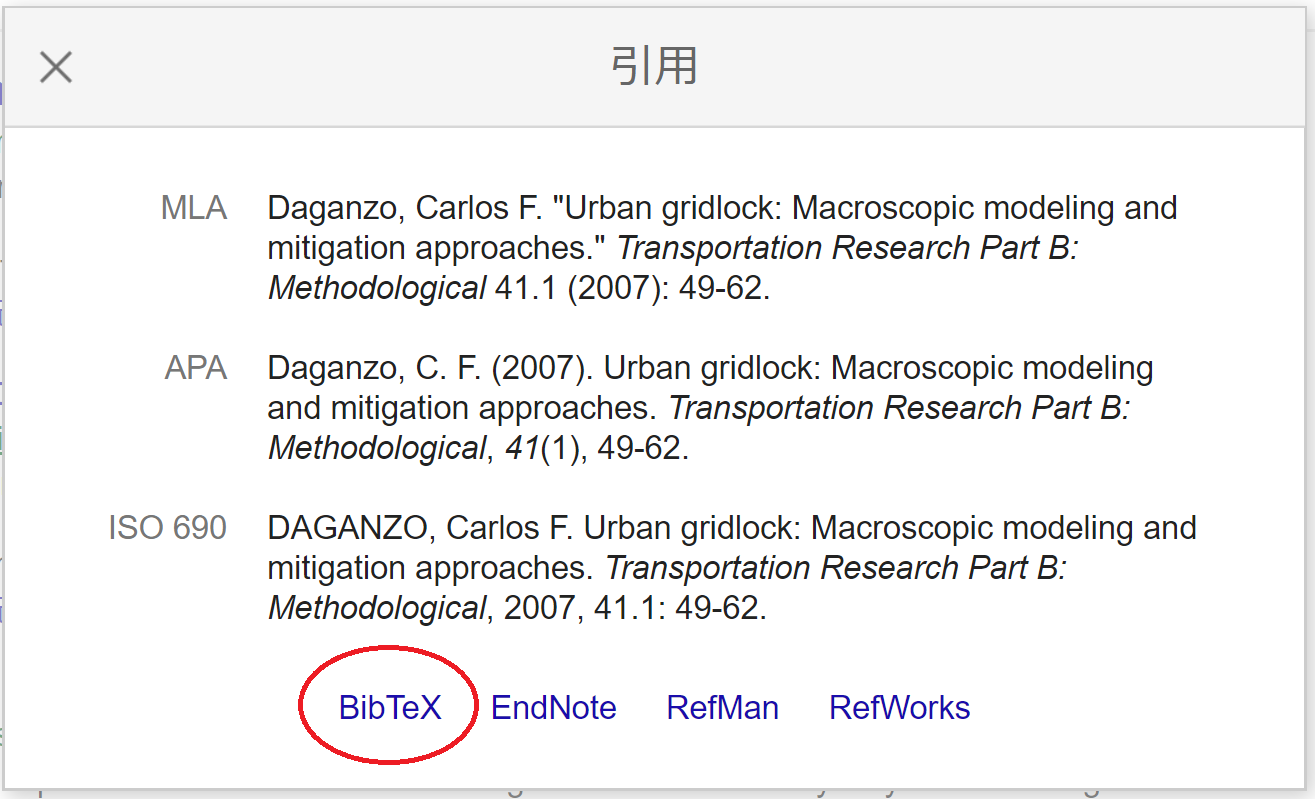
\includegraphics[clip, width=0.5\columnwidth]{image/bib2.png}
  \label{fig:bib1}
\end{figure}
\par
すると,以下のようなコードが記述された別ページに遷移する.
\begin{figure}[!ht]
  \centering
  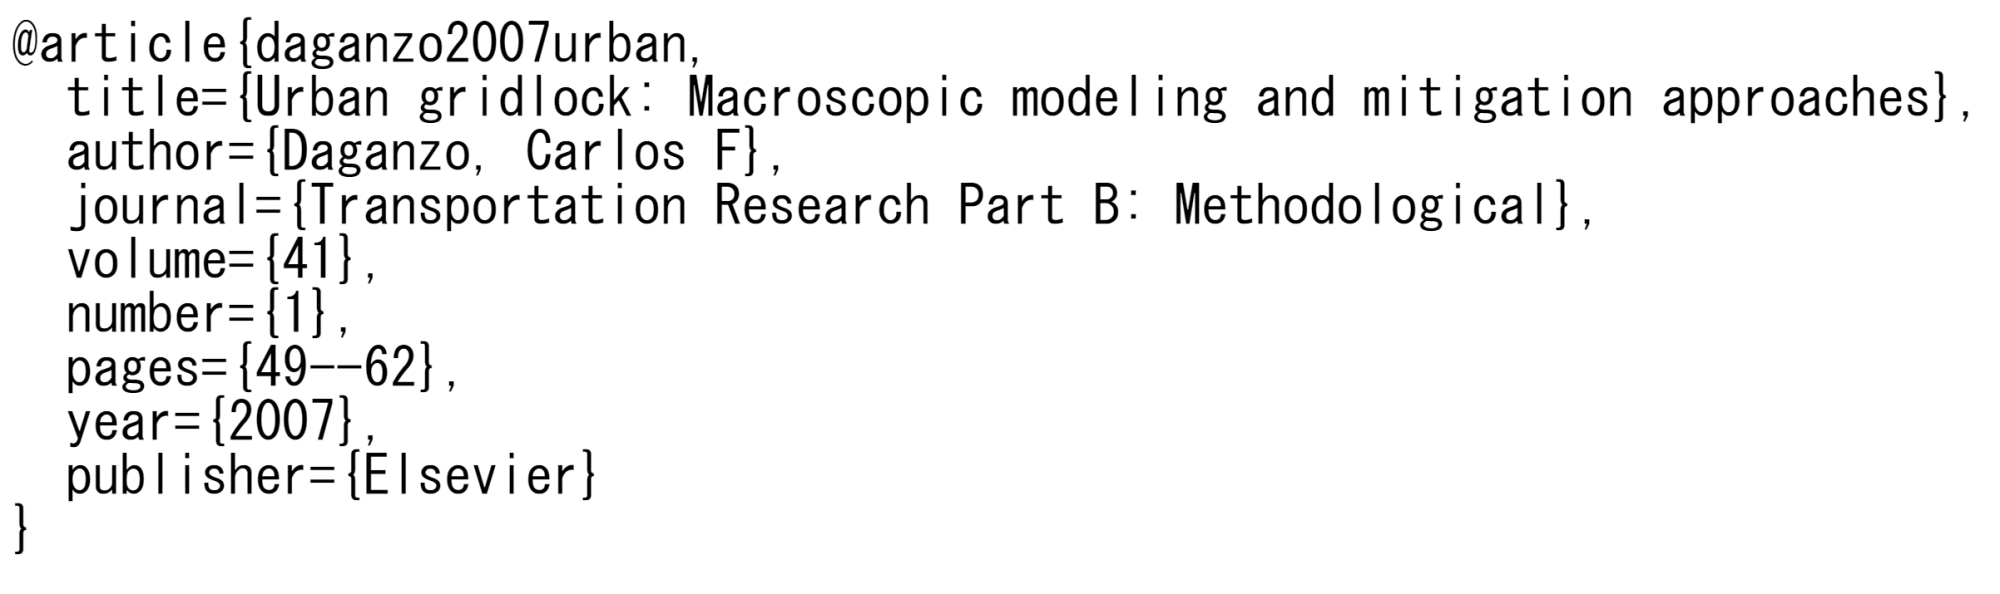
\includegraphics[clip, width=0.5\columnwidth]{image/bib3.png}
  \label{fig:bib1}
\end{figure}
\par
これをコピーして,refs.bibに貼り付ける.

\subsection{本文内での引用}
本文内での引用は\verb|\cite{キー}|を用いて行う.
例えば,\verb|\citet{Vickrey1969-ic}|と記述すると,\citet{Vickrey1969-ic}となる.
その他,\verb|\citep|,\verb|\citeauthor|,\verb|\citeyear|などがある.
詳しくは,\url{https://www.overleaf.com/learn/latex/Natbib\_citation\_styles}を参照のこと.

\subsection{文献管理ツール}
Google Scholarで一つずつ文献を引用するのは面倒である.
世の中には様々な文献管理ツールがあり,これらを用いることで簡単に文献を管理することができる.
また,一括でbibファイルを出力することもできる.
\begin{itemize}
  \item Paperpile
  \item JabRef
  \item Mendeley
  \item Zotero
  \item EndNote
  \item Citavi
\end{itemize}
おすすめは,Paperpileであるが,月2.99ドルかかる.

\newpage
\section{図の挿入}
図はpng, pdf, eps, jpgなどの画像ファイルを用いて挿入する.pdfがおすすめ.
\par
図の挿入は,figure環境を用いて行う.
\begin{lstlisting}[language={[latex]TeX}]
  \begin{figure}[!ht]
    \center
    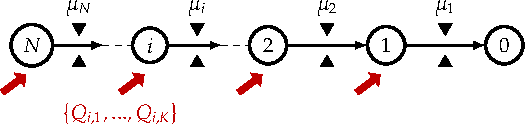
\includegraphics[clip, width=0.5\columnwidth]{image/sample.pdf}
    \caption{$N$個の起点からなるコリドーネットワーク}
    \label{fig:CorridorNetwork}
  \end{figure}
\end{lstlisting}
\begin{figure}[!ht]
  \center
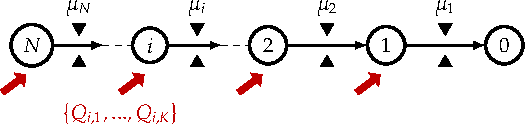
\includegraphics[clip, width=0.5\columnwidth]{image/sample.pdf}
  \caption{$N$個の起点からなるコリドーネットワーク}
  \label{fig:CorridorNetwork}
\end{figure}

\newpage
\section{表の挿入}
表は作成は次のように記述する.
\lstset{
    frame=single,
    numbers=left,
    tabsize=2
}
\begin{lstlisting}[language={[latex]TeX}]
  \begin{table}[ht]
    \centering % 表を中央揃えにする
    \caption{サンプルテーブル} % 表のタイトル
    \label{tab:sample_table} % 表を参照するためのラベル
    \begin{tabular}{lcr} % 列の配置: left, center, right
    \toprule % 上部の罫線
    列1のヘッダ & 列2のヘッダ & 列3のヘッダ \\
    \midrule % 中間の罫線
    行1のデータ1 & 行1のデータ2 & 行1のデータ3 \\
    行2のデータ1 & 行2のデータ2 & 行2のデータ3 \\
    行3のデータ1 & 行3のデータ2 & 行3のデータ3 \\
    \bottomrule % 下部の罫線
   \end{tabular}
  \end{table}
\end{lstlisting}
これをコンパイルすると,次のようになる.
\begin{table}[ht]
  \centering % 表を中央揃えにする
  \caption{サンプルテーブル} % 表のタイトル
  \label{tab:sample_table} % 表を参照するためのラベル
  \begin{tabular}{lcr} % 列の配置: left, center, right
  \toprule % 上部の罫線
  列1のヘッダ & 列2のヘッダ & 列3のヘッダ \\
  \midrule % 中間の罫線
  行1のデータ1 & 行1のデータ2 & 行1のデータ3 \\
  行2のデータ1 & 行2のデータ2 & 行2のデータ3 \\
  行3のデータ1 & 行3のデータ2 & 行3のデータ3 \\
  \bottomrule % 下部の罫線
 \end{tabular}
\end{table}

\newpage
\section{数式}
数式は,align環境を用いて記述すると良い.
\begin{align}
  &y = a x^{2} + bx + c
  \\
  &\VtA = 
  \begin{bmatrix}
    1 & 2 & 3 \\
    4 & 5 & 6 \\
    7 & 8 & 9
  \end{bmatrix}
  \\
  &\begin{dcases}
    F(x) = 0 &\text{if}   \quad x>0
    \\
    F(x) \geq 0 &\text{if} \quad x=0
  \end{dcases}
\end{align}
\section{定理環境}
定義,仮定,定理,命題,補題,系などは,\verb|amsthm|パッケージを用いて記述する.
\begin{dfn}[凸集合]
  集合 $\ClS \subset \mathbb{R}^n$ が凸集合であるとは,任意の $x, y \in \ClS$ と任意の $\lambda \in [0, 1]$ に対して,$\lambda x + (1 - \lambda) y \in \ClS$ が成り立つことをいう.
\end{dfn}
\begin{thm}[角谷の不動点定理]
  \label{thm:Kakutani}
  $S$ を,ユークリッド空間 $\mathbb{R}^n$ の空でないコンパクト凸部分集合とする.$\varphi: S \rightarrow 2^S$ を $S$ 上の集合値関数で,閉グラフと次の性質を備えるものとする:$\varphi(x)$ は $x \in S$ に対して空でない凸集合である.
  このとき,$\varphi$ は不動点を持つ.
\end{thm}



\newpage
\section{アルゴリズム}
アルゴリズム(疑似コード)は,algorithm, algpseudocodeパッケージを用いて記述する.詳しい使い方は,\url{https://www.overleaf.com/learn/latex/algorithms}を参照のこと.
\begin{lstlisting}[language={[latex]TeX}]
  \begin{algorithm}[ht]
    \caption{サンプルアルゴリズム}
    \label{alg:sample_algorithm}
    \begin{algorithmic}[1]
      \Require $x$,$y$
      \Ensure $z$
      \State $z \gets x + y$
      \State \Return $z$
    \end{algorithmic}
  \end{algorithm}
\end{lstlisting}
\begin{algorithm}[!ht]
  \caption{サンプルアルゴリズム}
  \label{alg:sample_algorithm}
  \begin{algorithmic}[1]
    \Require $x$,$y$
    \Ensure $z$
    \State $z \gets x + y$
    \State \Return $z$
  \end{algorithmic}
\end{algorithm}

\section{付録の挿入}
付録は,subappendices環境を用いて挿入する.
\begin{lstlisting}[language={[latex]TeX}]
  \begin{subappendices}
    \section\{証明\}
    ここは章ごとの付録.
  \end{subappendices}
\end{lstlisting}


\newpage
\section{FAQ}
\subsection*{まずは...}
  \begin{itemize}
    \item コンパイルエラーの多くは,エラーメッセージをそのままググることで,解決策が見つかることが多い.まずは,エラーメッセージをググること.chatgptに聞くのも良い.
    \item 一時ファイルを削除してからコンパイルすると,エラーが解消されることがある.
  \end{itemize}

\subsection*{Q1. 参考文献を出力したいが,subfileごとに出力されてしまう}
main.texの\verb|\bibdummy{1}|を\verb|\bibdummy{0}|に変更する.

\subsection*{Q2. 章番号がずれている}
サブファイルの冒頭の\verb|\setcounter{chapter}{n}|を,章番号-1の値に変更する.


\bibdummy{1}% {1}にするとsubfileごとのコンパイルでも参考文献を出力する.{0}にすると出力しない.
\end{document}
